\documentclass[11pt]{scrartcl}
\usepackage[scale=1.5]{ccicons}
\usepackage[notextcomp]{kpfonts} 
\usepackage[margin=1.0in]{geometry}
\usepackage{amsthm,amssymb,amsmath}
\usepackage{graphicx}
\usepackage{subcaption}
\usepackage{enumitem}
\usepackage{bm}
\usepackage{tabu}
\usepackage{mathtools}
\usepackage{tikz}
\usepackage{tikz-3dplot}
\usepackage{xcolor}
\usepackage{colortbl}
\usepackage{wasysym}
\usepackage{tabularx}


\newcolumntype{C}{>{\raggedright\arraybackslash $}X<{$}}



\usepackage{color}
\definecolor{darkblue}{rgb}{0, 0, .6}
\definecolor{grey}{rgb}{.7, .7, .7}
\usepackage[breaklinks]{hyperref}
\hypersetup{
	colorlinks=true,
	linkcolor=darkblue,
	anchorcolor=darkblue,
	citecolor=darkblue,
	pagecolor=darkblue,
	urlcolor=darkblue,
	pdftitle={},
	pdfauthor={}
}
\usepackage{fancyhdr}
\thispagestyle{fancy}
\lhead{Math 112}
\chead{Lesson Plans}
\rhead{Spring 2018}
%\lfoot{}%\scriptsize This work is licensed under the \href{http://creativecommons.org/licenses/by-sa/3.0/us/}{Creative Commons Attribution-Share Alike 3.0 License}.} 
%\cfoot{}
%\rfoot{\ccbysa}
\renewcommand{\headrulewidth}{.4pt}
%\renewcommand{\footrulewidth}{.4pt}

\theoremstyle{definition}
\newtheorem{theorem}{Theorem}
\newtheorem*{theorem*}{Theorem}
\newtheorem{acknowledgement}[theorem]{Acknowledgement}
\newtheorem{algorithm}[theorem]{Algorithm}
\newtheorem{axiom}[theorem]{Axiom}
\newtheorem{case}[theorem]{Case}
\newtheorem{claim}[theorem]{Claim}
\newtheorem*{claim*}{Claim}
\newtheorem{conclusion}[theorem]{Conclusion}
\newtheorem{condition}[theorem]{Condition}
\newtheorem{conjecture}[theorem]{Conjecture}
\newtheorem{corollary}[theorem]{Corollary}
\newtheorem{criterion}[theorem]{Criterion}
\newtheorem{definition}[theorem]{Definition}
\newtheorem{example}[theorem]{Example}
\newtheorem{exercise}[theorem]{Exercise}
\newtheorem{journal}[theorem]{Journal}
\newtheorem{lemma}[theorem]{Lemma}
\newtheorem{notation}[theorem]{Notation}
\newtheorem{problem}[theorem]{Problem}
\newtheorem*{problem*}{Problem}
\newtheorem{proposition}[theorem]{Proposition}
\newtheorem{remark}[theorem]{Remark}
%\newtheorem{solution}[theorem]{Solution}
\newtheorem{summary}[theorem]{Summary}
\newtheorem{skeleton}[theorem]{Skeleton Proof}
\newtheorem{activity}[theorem]{Activity}
\newtheorem{intuitivedef}[theorem]{Intuitive Definition}

\DeclareMathOperator{\spn}{span}
\DeclareMathOperator{\Char}{Characteristic}
\DeclareMathOperator{\Aut}{Aut}
\DeclareMathOperator{\stab}{Stab}
\DeclareMathOperator{\Stab}{Stab}
\DeclareMathOperator{\orb}{\mathcal{O}}
\DeclareMathOperator{\lcm}{lcm}
\DeclareMathOperator{\gl}{GL}
\DeclareMathOperator{\Ker}{Ker}
\DeclareMathOperator{\Z}{\mathbb{Z}}
\DeclareMathOperator{\C}{\mathbb{C}}
\DeclareMathOperator{\R}{\mathbb{R}}
\DeclareMathOperator{\N}{\mathbb{N}}
\DeclareMathOperator{\Q}{\mathbb{Q}}
\DeclareMathOperator{\A}{\mathbb{A}}
\DeclareMathOperator{\Gal}{Gal}
\DeclareMathOperator{\PS}{\mathcal{P}}
\DeclareMathOperator{\acc}{acc}


\newenvironment{solution}{\begin{proof}[Solution]}{\end{proof}}
\newcommand{\comment}[1]{%
  \text{\phantom{(#1)}} \tag{#1}
}


%Useful for cut and paste
%\begin{enumerate}[label=\rm{(\alph*)}]

\begin{document}
%%%%%%%%%%%%%%%%%%%% Functions %%%%%%%%%%%%%%%%%%%%%%%%
%\section*{Functions}
%	\subsection*{Introductory Example}
%	In a certain city, sales tax is 9\%. Write an expression to express the total cost of purchasing as an item with selling price of $x$ dollars, after tax is added.
%	\bigskip\\
%		\hangindent=1.cm \hangafter=2
%			Students work on this with their elbow buddy.\\
%			Questions to ask students:
%			\begin{enumerate}[leftmargin=!,labelindent=1.5cm,itemindent=-15pt]
%				\item What is the total cost of an item with a selling price of \$40? \$200? How do you know?
%				\item Using the expression you created, how do you find the sales tax on any item?
%				\item What are the possible values that we can plug into this expression for $x$?
%				\item We say that tax is a function of the selling price of the item. How can we denote this using function notation?
%				\item The domain of a function is the set of all possible input values. What is the implied domain of this particular function?
%			\end{enumerate}
%		
%	\subsection*{Things you need to know about functions}
%		Students work in groups to discuss what they know about functions. Give about 3-5 minutes for them to discuss and write down what they know. Share as a class. 
%		\noindent
%		To make sure all bases are covered make sure the following questions are answered:
%		\begin{enumerate}
%			\item What is the definition of a function? (A function is a relationship between two variables, an input variable (often $x$) and an output variable (often $y$) in such a way that for every value of the input variable there is exactly one corresponding value of the output variable.)
%			\item What is meant by an input (or independent) variable? An output (or dependent) variable?
%			\item What is function notation and how do we use it?
%			\item What is meant by the domain of a function? (the set of all values of the input variable for which the funciton is defined in the real number system and in the case of an application problem in which the context makes sense) Range of a function? (the set of values of the dependent variable (easiest to identify from a graph))
%			\item How can you identify whether an equation, graph, or table of values represents a function?
%			\item If we restrict ourselves to functions whose output values are real numbers, what restrictions would we have to impose on the domain (what kinds of expressions might cause us trouble)?
%		\end{enumerate}
%		\noindent
%		Create a cohesive document about what they need to identify about functions \textbf{This should be emphasized as something that needs to go into their notes!}
%	
%	\subsection*{Example 1}
%		As you drive at a fairly constant speed of approximately 60 mph from Tucson to Bisbee (94 miles) you pass through Benson, which is 40 miles from Tucson. Sketch a graph of your distance from Tucson against time. Indicate on your graph the time when you reach Benson.
%		\bigskip \\
%		\hangindent=1cm \hangafter=3
%		Have students work on this individually at first.\\
%		Come back as a class and create a good model for them (read the context, determine what ``x" and ``y" are, determine domain and range, label axes, scale to make it understandable and label critical points in some way)
%		\hangindent=1cm \hangafter=0
%		Questions to ask students:
%		\begin{enumerate}[leftmargin=!,labelindent=1.5cm,itemindent=-15pt]
%				\item What is the input variable? Output variable?
%				\item What is an appropriate domain and range?
%				\item What labels should be put on the axes? What scale can/should be used?
%				\item Does this graph represent a function? How do you know? Why does this make sense?
%				\item What are the intercepts of this graph, and what do they represent?
%				\item Challenge: What if we looked at a different relationship, like distance from Benson/Bisbee as a function of time? Draw then new graph.
%		\end{enumerate}
%		\textbf{Is there anything we need to add to our notes about identifying functions?}
%	\subsection*{Example 2}
%	The following table shows market data that a sunglass manufacturer has gathered on a particular pair of sunglasses:
%		\begin{center}
%		\begin{tabular}{|l|l|l|l|l|l|}
%		\hline
%		Purchase Price                                      & \$46   & \$40   & \$37   & \$30   & \$27   \\ \hline
%		Consumer demand (quantity purchased) & 16,000 & 40,000 & 52,000 & 80,000 & 92,000 \\ \hline
%		\end{tabular}
%		\end{center}
%		Does this table represent the demand as a function of the price? Why or why not? Does it represent the price as a function of the demand? Why or why not?
%		\bigskip\\
%		\hangindent=1cm \hangafter=2
%		Students work on this in the pairs.\\
%		Come back and share as a class.\\ 
%		Questions to ask students:
%		\begin{enumerate}[leftmargin=!,labelindent=1.5cm,itemindent=-15pt]
%			\item Does this table represent a function? How do you know? How does this fit with our definition of function? How does it fit with the vertical line test?
%			\item What is an appropriate domain and range for this function?
%		\end{enumerate}
%		
%		\textbf{Is there anything we need to add to our notes about identifying functions?}
%		
%	\subsection*{More Practice}
%	For each of the following, determine the domain of the function, and evaluate $g(2)$ and $g(a+3)$.
%	\begin{enumerate}
%		\item $g(x)=3x^2-5x$
%		\item $g(x)=\frac{2x-1}{x+3}$
%		\item $g(x)=\sqrt{2-5x}-1$
%	\end{enumerate}
%	
%	\noindent
%	For the function $f(x)=3x^2-5x$, find $\frac{f(h+4)-f(4)}{h}$.	
%	
%	%The More Practice section became a warm up section (the problems were split over two days-see the print offs area). Example 2 also became a warm-up problem.
%
%%%%%%%%%%%%%%%%%%% Graphs %%%%%%%%%%%%%%%%%%%%%	

%\section*{Graphs}
%\subsection*{Introductory Example}
%A business has determined a mathematical model based on market data for its profit, $P$ (in dollars) as a function of the number of items sold, $x$. The model is given by the function $P(x)=-0.1x^2+150x-14,000$. Graph this function in an appropriate viewing window. Use the graph to determine the number of items that should be produced and sold in order to maximize profit.\\
%
%\noindent
%Questions to ask students before graphing:
%\begin{enumerate}
%	\item What is meant by profit? How does it differ from other related terms, like revenue and cost?
%	\item How do you know this is a function?
%	\item What is an appropriate viewing window? What does this mean?
%	\item What things will be helpful to us in determining an appropriate viewing window?
%	\end{enumerate}
%
%\noindent
%Things that students should touch on as helpful in determining and appropriate viewing window:	
%\begin{enumerate}
%	\item What is the natural restriction on $x$, based on the context of the problem?
%	\item What is $P(50)$, and what does this tell you in practical terms?		
%	\item Find the vertical intercept ($y$-intercept). What does this tell you? How can this help you to set the appropriate viewing window?
%	\item How can the TABLE feature on the calculator help us to set the appropriate viewing window?
%\end{enumerate}
%
%\noindent	
%Things to talk about once we have the graph in front of us:	
%\begin{enumerate}
%	\item Based on the graph, what are the $x$-intercepts of the function? What do they tell you? How could you find them algebraically?
%	\item On what interval(s) is the function negative? Positive? What does this tell you in practical terms?
%	\item On what interval is the function increasing? Decreasing? What does this tell you in practical terms?
%	\item What is the set of allowable inputs (domain)? What is the set of possible outputs (range)?
%\end{enumerate}
%
%\subsection*{Things to know about graphs of functions:}
%\begin{itemize}
%	\item Domain: Set of all values of input variable
%	\item Range: Set of all values of output variable
%	\item Increasing on: open interval on which the graph is rising from left to right \textbf{Always get from the graph!}
%	\item Decreasing on: open interval (x-values) on which the graph is falling from let to right
%	\item Constant on: open interval (x-values) on which a graph is neither rising nor falling
%	\item Positive on: open interval (x-values) on which the graph is above the x-axis
%	\item Negative on: open interval (x-values) on which the graph is below the x-axis
%	\item x-intercepts: points for which $f(x)=0$, graph intersects the $x-axis$
%	\item y-intercepts: point the graph intersects the $y-axis$ ($y$-value for when $x=0$)
%\end{itemize}
%
%\subsection*{Example 1}
%A cup of coffee that is initially $150^\circ$ F is placed in a room kept at a constant $72^\circ$ F. The temperature of the coffee, $T$ as a function of time is given by $T(x)=72+79e^{-0.223x}$, where $x$ is measured in minutes. Graph the function $T(x)$ in an appropriate viewing window. Use the graph to determine the timeframe during which the coffee is at a good drinking temperature, between $120^\circ$ F and $140^\circ$ F.\\
%
%\noindent
%Questions to ask students before graphing:
%\begin{enumerate}
%	\item What is $e$? How do we find the value of $e$ on our calculator?
%\end{enumerate}
%
%\noindent
%Questions to ask while graphing:
%\begin{enumerate}
%	\item What are the key pieces of information that help you determine which window to use? What is an appropriate window?
%	\item Find the intercepts what do they tell you in practical terms?
%	\item What is the domain? The range? What do they tell you in practical terms?
%	\item On what intervals(s) is the function increasing? Decreasing? Why does this make sense?
%\end{enumerate}
%
%\subsection*{Example 2}
%The cost, $C$ (in thousands of dollars), of removing $x$ percent of a certain pollutant from a lake is given by the formula $C(x)=\frac{18x}{100-x}$. Graph this function in an appropriate window.\\
%
%\noindent
%Questions to ask before graphing:
%\begin{enumerate}
%	\item What is the domain of the function?
%\end{enumerate}
%
%\noindent
%Questions to ask while graphing:
%\begin{enumerate}
%	\item What is the range? What does this tell us in practical terms?
%	\item Find the intercept(s). What does that tell us in practical terms?
%	\item On what interval(s) is the function increasing? Decreasing? Why does this make sense?
%\end{enumerate}
%
%\subsection*{More Practice}
%Determine the domain, range, and intercepts of each function. Determine the intervals on which the function is increasing/decreasing/constant, and on which the function is positive/negative.
%\begin{enumerate}
%	\item $g(x)=\sqrt{2x-5}-1$
%	\item $T(x)=x^3-4x$
%\end{enumerate}

%%%%%%%%%%%%%%%%%%%%%%%% Linear %%%%%%%%%%%%%%%%%%%%%%%%%%%

%\section*{Linear Equations}
%\subsection*{Introductory Example}
%A company produces a pair of skates for \$43.53 and sells each pair for \$89.95. The fixed costs incurred regardless of the number of skates produced are \$742.72. 
%\begin{itemize}
%	\item Write the total cost as a function of the number of pairs of skates produced.
%	\item Write the revenue as a function of the number of pairs of skates produced/sold.
%	\item Graph these two functions on the same set of axes. Indicate your viewing window. Think about an appropriate domain for this context.
%\end{itemize}
%
%\noindent
%Questions to ask the students before we start:
%\begin{enumerate}
%	\item What is meant by fixed costs? Total cost? Revenue?
%	\item What kind of functions are the cost and revenue? How do you know?
%	\item What is the general form of this type of function? What do each of the parts of the equation represent?
%\end{enumerate}
%Questions to ask as the students work:
%\begin{enumerate}
%	\item In this case, what is the slope of the cost function? The revenue function? What do these represent? Why is it important that the slope of the revenue function be greater than the slope of the cost function?
%	\item What is the $y$-intercept of each of these functions? What do they represent.
%	\item Graph both functions on the same set of axes in an appropriate window.
%	\item Where do these functions intersect? How can you find this point algebraically? Graphically? What does this point represent?
%\end{enumerate}
%
%\subsection*{Things to know about linear functions}
%\textbf{General form of a function} $f(x)=mx+b$ where $m=$slope and $b=y$-intercept\\
%
%\noindent
%\textbf{Slope:} positive slope, negative slope, horizontal line, vertical line, units of slope, finding the slope
%
%\noindent
%\textbf{How to find the slope of the line through two points}
%
%\subsection*{Strategies and Understanding a New Context}
%\textbf{Strategies}\\
%\begin{enumerate}
%	\item Identify input/output
%	\item Make a table
%	\item Identify domain
%	\item Formula
%	\item Graph
%\end{enumerate}
%
%\noindent
%\textbf{Understanding a New Context}
%\begin{enumerate}
%	\item Do you know all the words?
%	\item Do you know how this function works? Try some points.
%	\item Use: 
%	\begin{itemize}
%		\item your brain - what do you already know?
%		\item the context - what clues/numbers are given?
%		\item the calculator/graph
%	\end{itemize}
%\end{enumerate}
%
%
%\subsection*{Example 1}
%A business bought a machine for \$25,000. After 4 years, the machine is valued at \$10,000. Assume the value of the machine depreciates linearly. Express the value of the machine as a function of time in years. Graph this function in an appropriate viewing window.\\
%
%\noindent
%Questions to ask students as they work:
%\begin{enumerate}
%	\item Is this a linear function? What cues help you to determine whether it is a linear function?
%	\item What is the input variable? What is the output variable?
%	\item What are the two ordered pairs that can be used to find the slope of this line?
%	\item What is the input variable measuring in this case? The output variable?
%	\item What is the slope? What are the units of slope? What does the slope represent in this case?
%	\item What are the intercepts and what do they represent? What is an appropriate domain for this function?
%\end{enumerate}
%
%\subsection*{Example 2}
%On most state highways, the fine for speeding depends on the speed of the car. In a certain state, the fine for driving 70 mph is \$25, and the fine for driving 85 mph is \$100. Assuming that this relationship is linear, write an equation for the fine as a function of the speed of the car.\\
%
%\noindent
%Questions to ask students as they work:
%\begin{enumerate}
%	\item What is the input variable? The out put variable?
%	\item What are the two order pairs that can be used to find the slope of this line?
%	\item What is the slope? What are the units of slope? What does slope represent in this case?
%	\item What is the $x$-intercept and what is the practical significance of this point?
%	\item What are the values of the independent variable for which this function is valid?
%\end{enumerate}
%
%\subsection*{Extra Practice}
%\begin{enumerate}
%	\item Determine an equation of the linear function passing through the points $(-4,5)$ and $(2,1)$.
%	\item Determine an equation in slope-intercept form for the linear function graphed below. Identify the intercepts.\\ \begin{center} 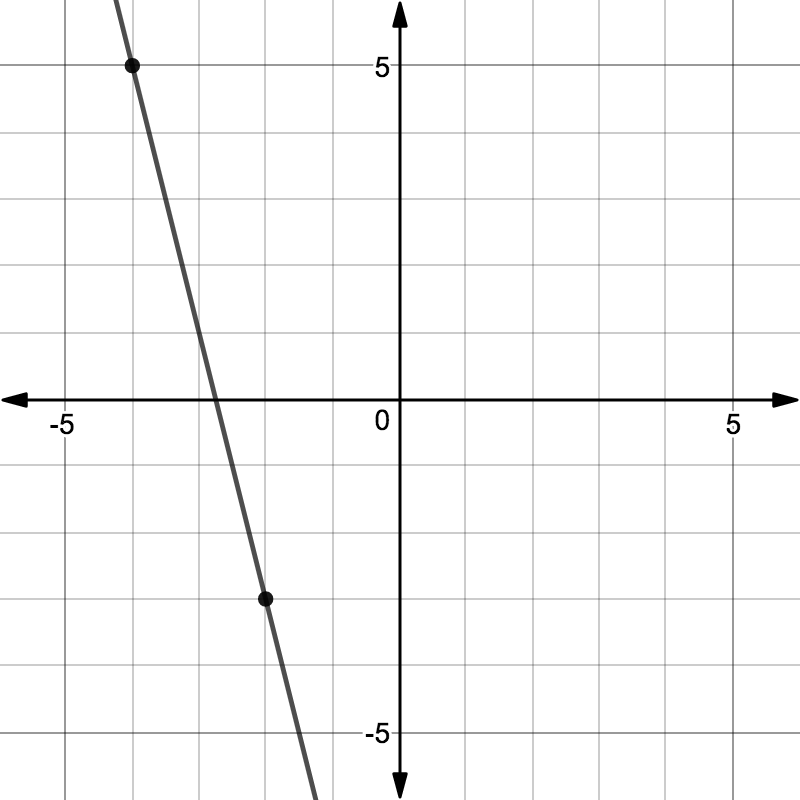
\includegraphics[scale=0.35]{Lineargraph} \end{center}
%\end{enumerate}

%%%%%%%%%%%%%%%%%%%%%%%% Piecewise Functions (Linear) %%%%%%%%%%%%%%%%%%%%%%%%%%%

%\section*{Piecewise Linear Functions}
%\subsection*{Introductory Example}
%A cell phone carrier charges \$50 per month per line, with 2gb of data included. Users who exceed 2gb of data are charged \$15 per gb over 2gb. Express the total monthly cost as a function of the number of gb of data used. Graph this function in an appropriate window.\\
%
%\noindent
%\begin{itemize}
%	\item Warm-up: the students will create a table of values and identify the input and output values 
%	\item Class to create a graph in an appropriate window by hand 
%	\item Students will come up with a function that represents the situation
%	\item Students will then identify the domain
%	\item Class discuss how to graph on a graphing calculator
%\end{itemize}
%
%\subsection*{Things to know about piecewise-defined linear functions:}
%Notation:\\
%Through an example: \[ f(x) = \begin{cases} 
% 2x-1 & \text{if } x <-2\\
% x+3 & \text{if } x \geq -2	
% \end{cases} \]
%
%\noindent
%Evaluation:\\
%Through the above example: Calculate $f(-3)$ and $f(1)$\\ 
%
%\noindent
%Graph:\\
%Through the above example\\
%
%\noindent
%Finding Intercepts:\\
%Through the above example (how many $x$-intercepts?, $y$-intercepts?)
%
%\subsection*{Example 1}
%A company is planning to order polo shirts pre-printed with their company logo from an online supplier. The cost to create the template for the logo is \$50. The cost per shirt is tiered, according to the number of shirts ordered. The cost per shirt is \$20 for up to 30 shirts. For orders of more than 30 shirts, the per shirt charge isn \$15. Write a function to represent the total cost of order $x$ shirts. Graph this function. If your total budget is \$1000 how many shirts can be ordered? What if the total budget is \$550?\\
%
%\noindent
%\begin{itemize}
%	\item Students write the equation on their own (then discuss)
%	\item Students graph the equation on the whiteboard in the appropriate fashion (then discuss)
%	\item Students then answer the questions (then discuss)
%\end{itemize}
%
%\subsection*{Example 2}
%For 2017, a single person whose taxable income is between \$0 - \$9,325 is charged 10\% in tax. A single person whose taxable income is between \$9,326 - \$37,950 is charged 10\% of the first \$9,325, and 15\% of the amount over \$9,325. Write a piecewise-linear function to represent the income tax for a single taxpayer as a function of taxable income, for taxable incomes up to \$37,950. Graph this function. If a person owes \$2,383.75 in federal income taxes, what is their taxable income?\\
%
%\noindent
%\begin{itemize}
%	\item Students write the equation for their own (then discuss)
%	\item Students graph the equation (then discuss)
%	\item Students answer the last question (then discuss)
%	\item For groups that finish early ask them to calculate their taxes based on the simplified bracket.
%\end{itemize}
%
%\subsection*{More Practice}
%For the function
%\[ f(x) = \begin{cases} -x-1 & \text{if } x \leq 2\\ 2x+3 & \text{if } x > 2 \end{cases} \]
%\begin{enumerate}[label=(\alph*)]
%	\item Find $f(-3)$, $f(2)$, $f(5)$
%	\item Graph the function
%	\item Find the intercepts	
%\end{enumerate}
%
%Find a rule (equation) for the function graphed below:
%\begin{center}
%	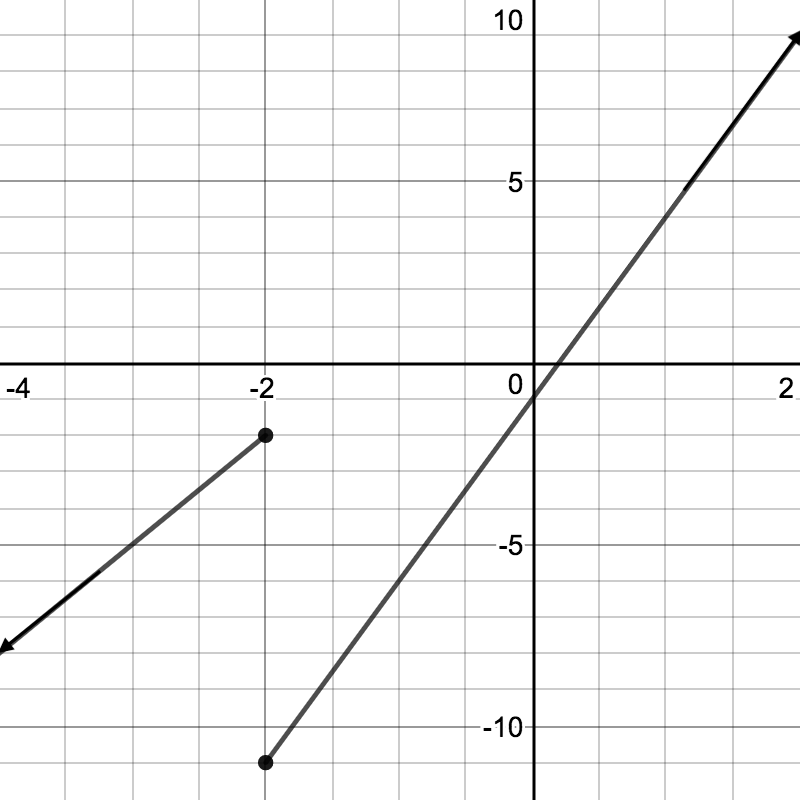
\includegraphics[scale=0.35]{piecewise1}
%\end{center}

%%%%%%%%%%%%%%%%%%%%%%%% Transformations %%%%%%%%%%%%%%%%%%%%%%%%%%%

%\section*{Transformations}
%\subsection*{Introductory Example}
%\begin{figure}[h!]
%\centering
%\begin{subfigure}{.5\textwidth}
%  \centering
%  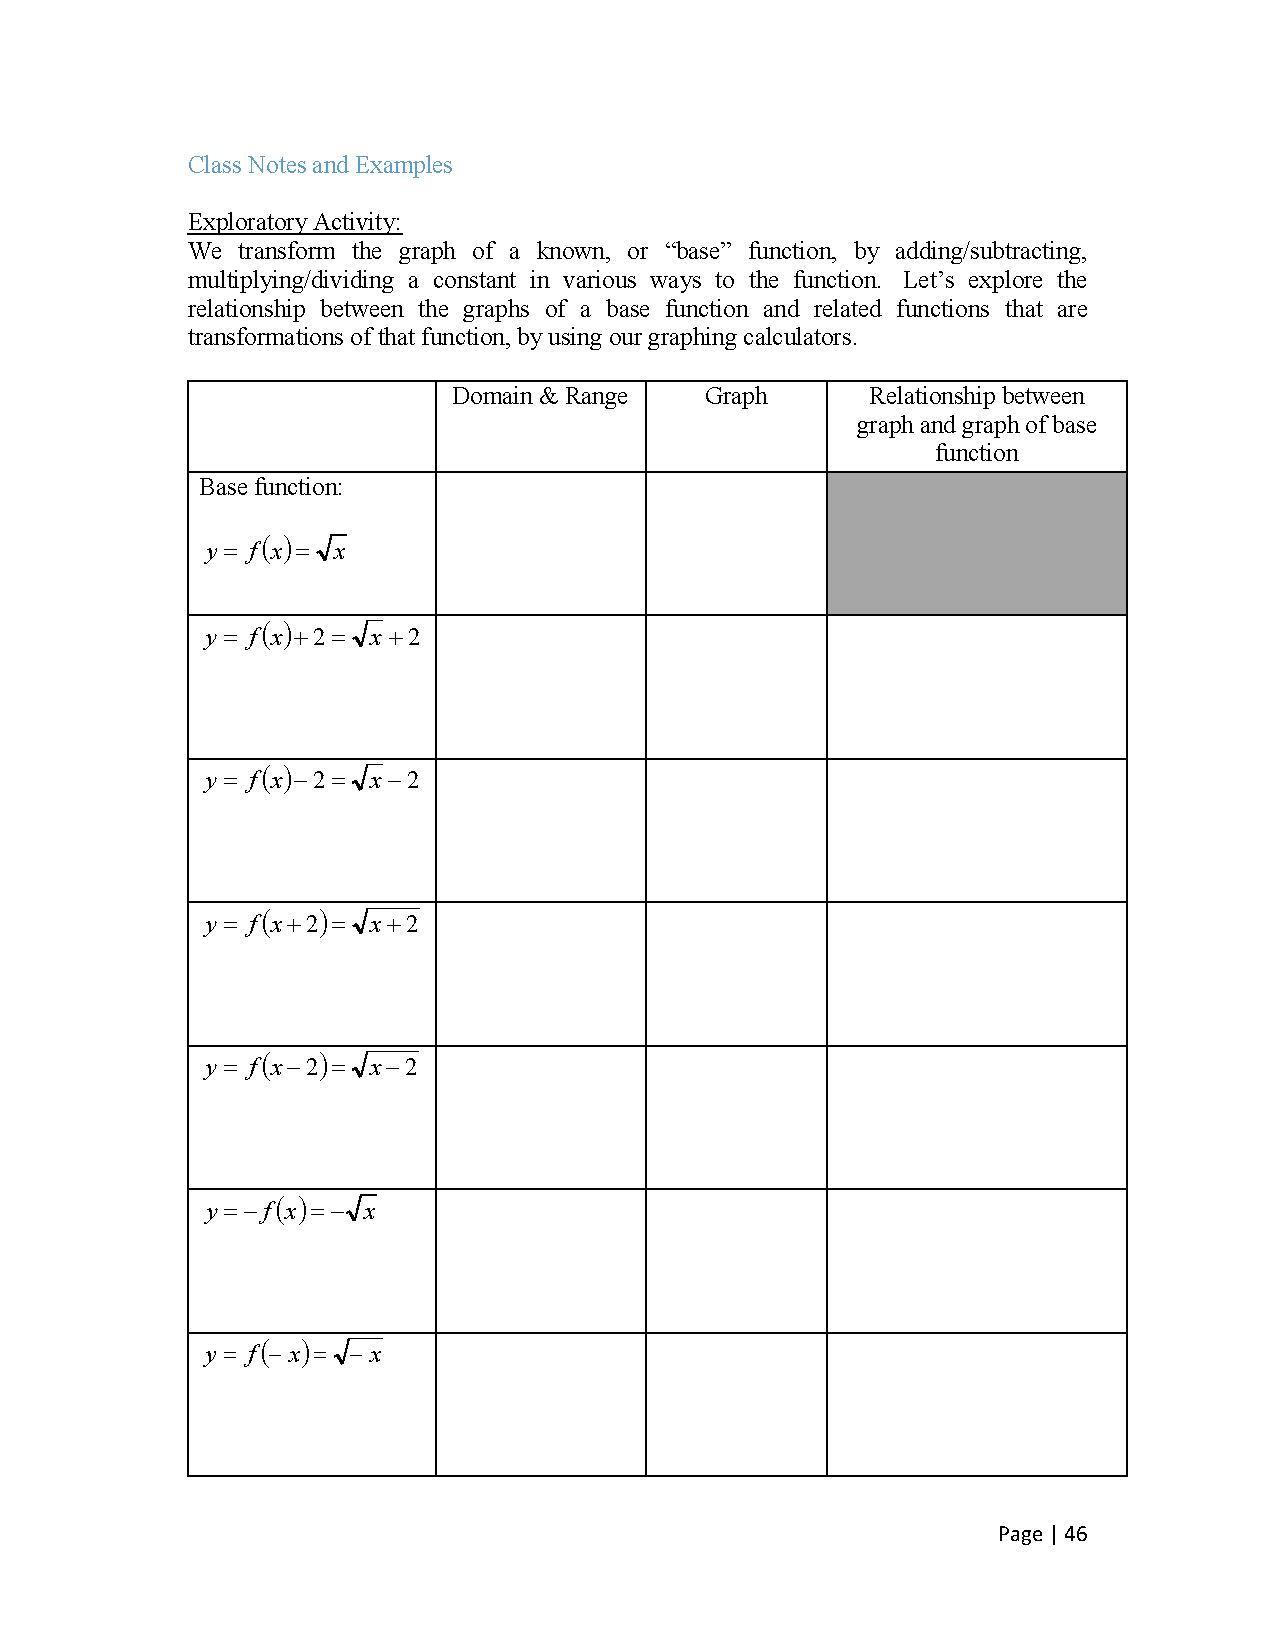
\includegraphics[scale=0.45]{TA1}
%\end{subfigure}%	
%\begin{subfigure}{.5\textwidth}
%  \centering
%  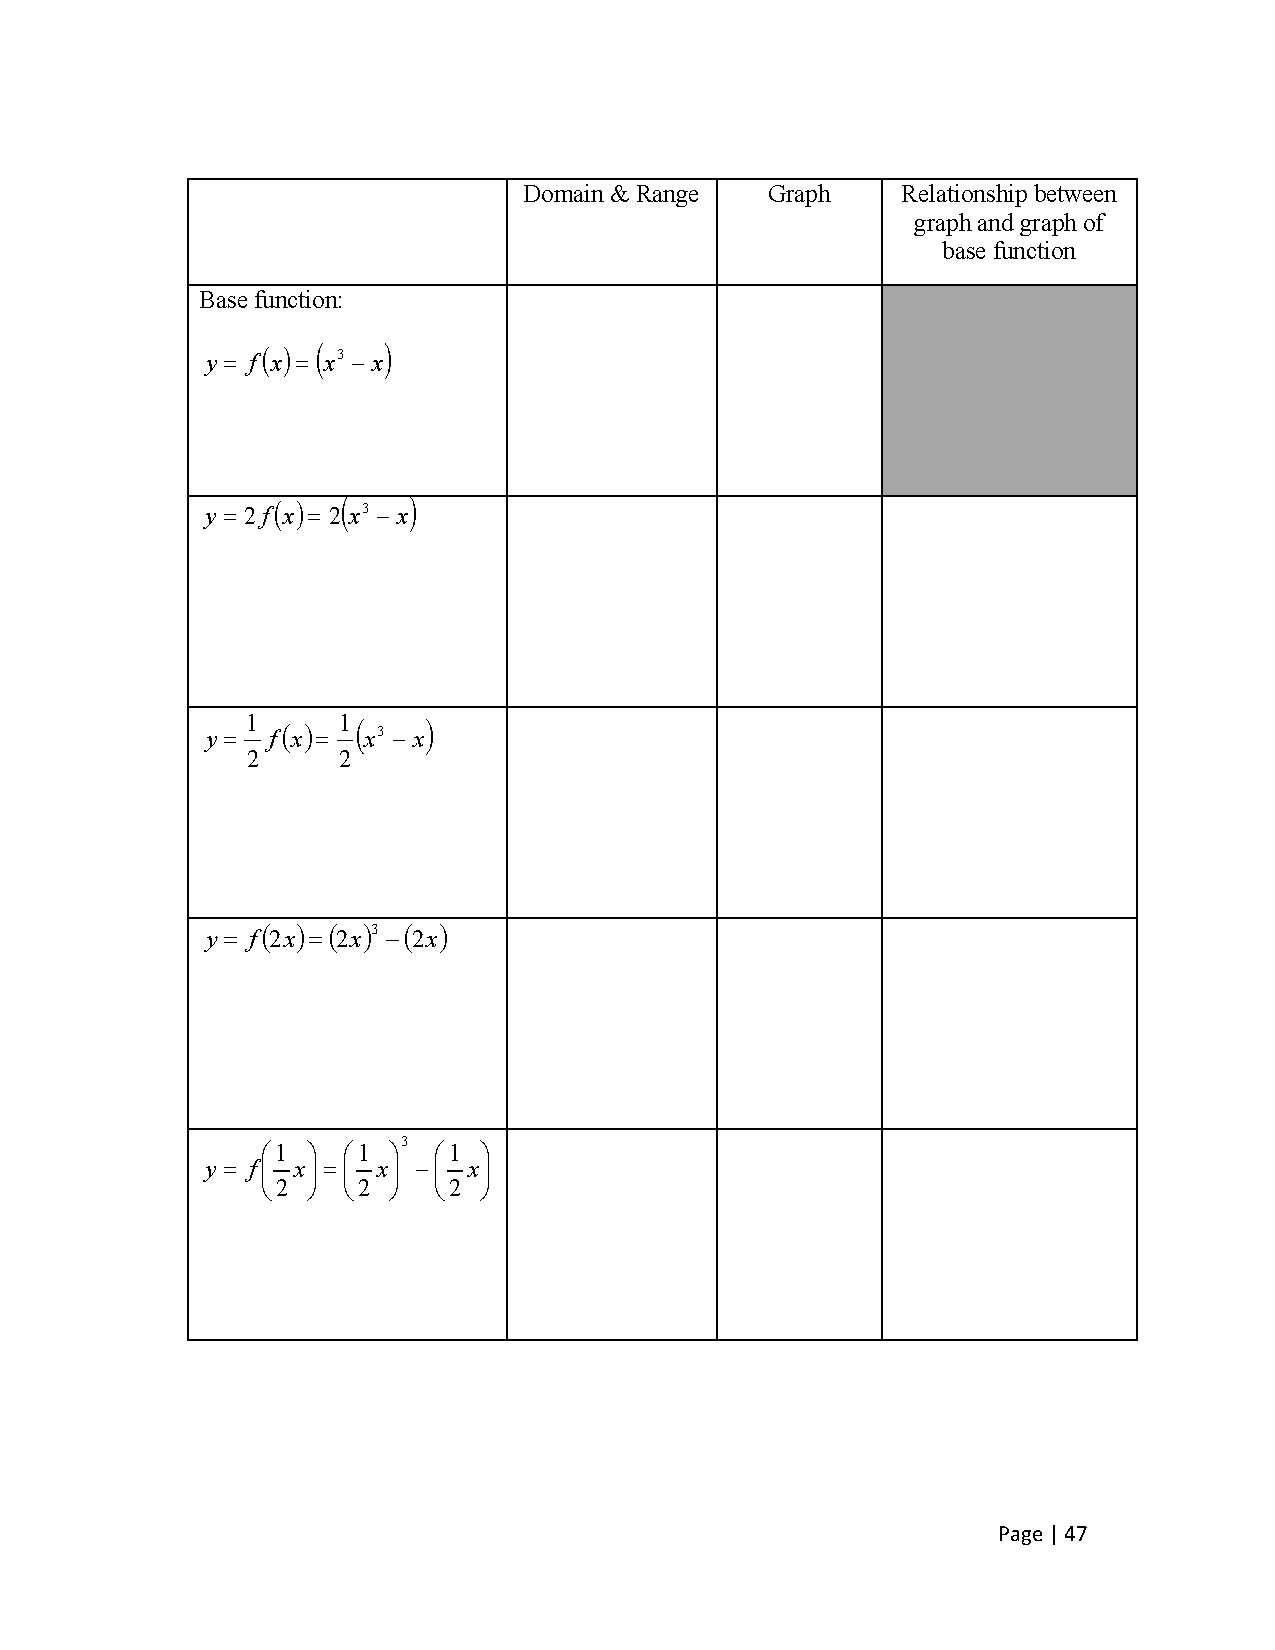
\includegraphics[scale=0.45]{TA2}
%\end{subfigure}
%\end{figure}
%
%\subsection*{Things to know about transformations}
%\begin{itemize}
%	\item $f(x)+C$, if $C$ is positive? Negative?
%	\item $f(x+C)$, if $C$ is positive? Negative?
%	\item $-f(x)$
%	\item $f(-x)$
%	\item $Cf(x)$, if $C>1$? if $0<C<1$?
%	\item $f(Cx)$, if $C>1$? if $0<C<1$?
%	\item Combining transformations: Show through examples: $-2f(x-5)+4$ and $\frac{1}{3} f(x+2) -4$
%\end{itemize}
%
%\subsection*{All About Graphs}
%The following is the graph of $y=f(x)$:\\
%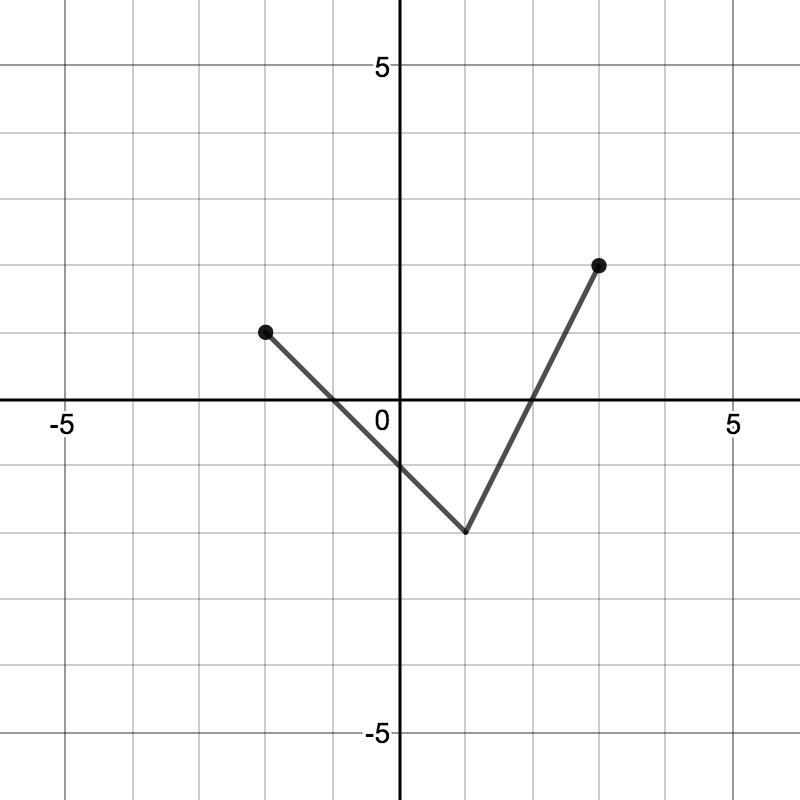
\includegraphics[scale=0.25]{transformations1}
%
%\noindent
%Use the above graph to answer the following questions:
%\begin{itemize}
%	\item What is the domain and range of $f(x)$?
%	\item Sketch the graph of $y=f(x)-2$ on the same set of axes. What are the domain and range of $f(x)-2$?
%	\item Sketch the graph of $y=f(x+3)$ on the same set of axes. What are the domain and range of $f(x+3)$?
%	\item Sketch the graph of $y=\frac{1}{2}f(x-1)$ on the same set of axes. What are the domain and range of $\frac{1}{2}f(x-1)$?
%\end{itemize}
%
%\vspace{1cm}
%
%\noindent
%The following is the graph of $y=g(x)$:\\
%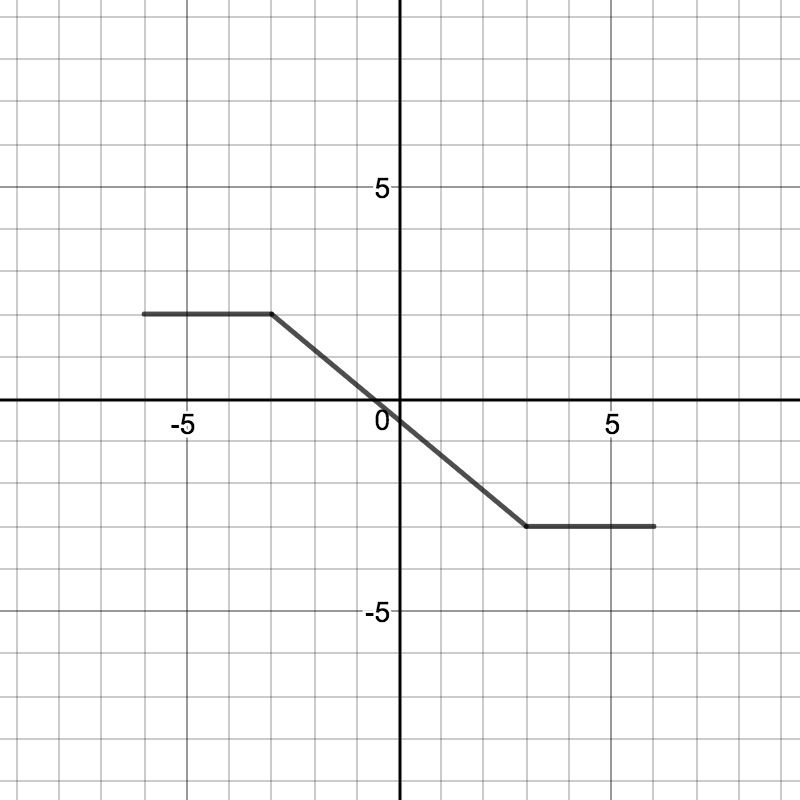
\includegraphics[scale=0.25]{transformations2}
%
%\noindent
%Use the above to answer the following questions
%\begin{itemize}
%	\item What is the domain and range of $g(x)$?
%	\item Sketch the graph of $y=2g(x+3)-1$ on the same set of axes. What are the domain and range of $2g(x+3)-1$?
%	\item Sketch the graph of $y=-g(\frac{1}{3}x)+3$ on the same set of axes. What are the domain and range of $-g(\frac{1}{3}x)+3$?
%	\item Sketch the graph of $y=g(-x)-4$ on the same set of axes. What are the domain and range of $g(-x)-4$?
%\end{itemize}
%
%\subsection*{Turning Transformations into words}
%For the following transformations identify the base function and describe the transformations in the appropriate order. Verify by graphing the equation.
%
%\begin{enumerate}
%	\item $y=(x-1)^3+4$
%	\item $y=-(x-2)^2+3$
%	\item $y=\frac{1}{2}(x+3)^4-5$
%	\item $y=3(\frac{1}{4}x)^2$
%	\item $y=-2\sqrt{x-5}+5$
%	\item $y=\sqrt{3x}-2$
%\end{enumerate}

%%%%%%%%%%%%%%%%%%%%%%%% Combining Functions %%%%%%%%%%%%%%%%%%%%%%%%%%%

%\section*{Combining Functions}
%\subsection*{Introductory Example}
%Recall this example from earlier in the semester. A company produces a pair of skates for \$43.53 and sells each pair for \$89.95. The fixed costs incurred regardless of the number of skates produced are \$742.72. We wrote the revenue, $R(x)$, and cost, $C(x)$ functions. Complete the following tasks:
%\begin{itemize}
%	\item Find $R(x)$ and $C(x)$.
%	\item Find the profit function $P(x)$.
%	\item Graph these three functions on the same set of axes.
%\end{itemize}
%
%\noindent
%Things to emphasize with the students:
%\begin{itemize}
%	\item The intersection of Revenue and Cost is the $x$-intercept for $P(x)$
%	\item What is $P(x)$? How do we find it? Mathematically how could we write this?
%\end{itemize}
%
%\subsection*{Comments for myself}
%Here we are doing a second example. The reason for this is that after the first day of lecture on this we have the first exam which won't cover this material. I don't want to overwhelm the students with new information so in doing the introductory example and the next example, we are practicing techniques that will be used on the test tonight. This way the students don't feel like today's lecture is shorting them on review time. In the next class we will continue in the typical format.
%
%\subsection*{Example 1}
%The local jazz society puts on a series of weekly concerts during the spring. When concert tickets are priced at \$15, the average attendance is 400 people. This past fall the society tried out different ticket prices and found that for every \$2 increase in ticket price, approximately 25 fewer people come to the show. \\
%
%\begin{itemize}
%	\item Write an equation to represent the attendance, $A(x)$, as a function of ticket price $x$.
%	\item Write a function that represents revenue generated by selling tickets as a function of the selling price $x$.
%	\item When (at what selling price) is revenue maximized?
%\end{itemize}
%
%\subsection*{Things to know about combining functions}
%\begin{itemize}
%	\item $(f+g)(x)=f(x)+g(x)$
%	\item $(f-g)(x)=f(x)-g(x)$
%	\item $(f\cdot g)(x)=f(x) \cdot g(x)$
%	\item $\frac{f(x)}{g(x)}$
%	\item $(f \circ g)(x)=f(g(x))$
%	\item $(g \circ g)(x)=g(f(x))$
%\end{itemize}
%
%\noindent
%Discuss the ``definition" of all the different ways to combine. Also discuss intuitively how to find the domain of these functions. This probably will come in the second class. This means that we can have a warm-up with the equations $f(x)=3x-1$ and $g(x)=\sqrt{5-2x}$ for the non-composition combinations.\\
%
%\subsection*{Example 2}
%The sales tax at a certain store is 9\%. 
%\begin{itemize}
%	\item Write a function for the total price paid, $P(x)$, for an item priced at $x$ dollars after factoring in sales tax. 
%	\item The store is having a sale and offering \$5 off every purchase. Write an equation, $S(x)$ for an item originally priced at $x$ dollars.
%	\item Find the composition $P(S(x))$.
%		\begin{itemize}
%			\item What does $P(S(x))$ represent?
%			\item Find $P(S(100))$. What does this mean in context of the problem?
%			\item Is $S \circ P$ the same thing as $P(S(x))$?
%			\item Does $S \circ P$ make sense in this context? Does it tell us anything useful?
%		\end{itemize}
%\end{itemize} 
%
%\subsection*{More Practice}
%\begin{enumerate}
%	\item Suppose $h(x)=\frac{3}{\sqrt{x-7}}$. What are two functions $f(x)$ and $g(x)$ such that $(f \circ g)(x)=h(x)$?
%	\item The following tables show the unemployment rate and crime rates in a certain city. Use these tables to answer some questions.
%		\begin{center}
%			\begin{tabular}{|l|l|}
%\hline
%$t$, time in years & $U$, unemployment rate \\ \hline
%0                  & 0.02                   \\ \hline
%1                  & 0.023                  \\ \hline
%1                  & 0.03                   \\ \hline
%3                  & 0.032                  \\ \hline
%\end{tabular}
%		\end{center} 
%		
%		\begin{center}
%			\begin{tabular}{|l|l|}
%\hline
%$U$, unemployment rate & Crime rate \\ \hline
%0.01                   & 0.015      \\ \hline
%0.02                   & 0.021      \\ \hline
%0.03                   & 0.028      \\ \hline
%0.04                   & 0.031      \\ \hline
%0.05                   & 0.037      \\ \hline
%\end{tabular}
%		\end{center}
%		
%\end{enumerate}

%%%%%%%%%%%%%%%%%%%%%%%% Inverse Functions %%%%%%%%%%%%%%%%%%%%%%%%%%%

%\section*{Inverse Functions}
%\subsection*{Introductory Example}
%Suppose that the demand for a certain pair of sunglasses can be expresses as a function of the purchase price using the equation $q=f(p)= -4000p+200,000$. Use this equation to answer these questions:
%\begin{enumerate}[label=(\alph*)]
%	\item What is the demand when the price is \$40?
%	\item What is $f(0)$ and what does this mean in practical terms?
%	\item Graph this function in a reasonable window.
%	\item What are the domain and range of this function?
%	\item What price corresponds to a demand of 80,000 pairs of sunglasses?
%\end{enumerate}
%
%\noindent
%After students work through these questions ask the students to express the price as a function of the quantity. Once they have completed this task ask these questions:
%\begin{enumerate}
%	\item Take your answer from part (a) and solve for the price. What happened? Why does this make sense?
%	\item When we solved for price as a function of the quantity, what were we doing?
%	\item What does an inverse function do for us?
%	\item How do we know that the function is an inverse? (Might use this for the next example?)
%\end{enumerate}
%
%\subsection*{Things you need to know about inverse functions}
%\begin{itemize}
%	\item When does a function have an inverse function?\\ \textit{A function is invertible if it is one-to-one, every output variable has exactly one input variable. Graphically it must pass the horizontal line test}
%	\item How do you find an inverse function, for a function that has one?\\ \textit{Solve for the input variable as a function of the output variable}
%	\item Notation:\\ \textit{If $y=f(x)$, then the inverse is denoted $x=f^{-1}(y)$}
%	\item Domain/Range:\\ \textit{The domain of $f^{-1}$ is the range of $f$. The range of $f^{-1}$ is the domain of $f$}
%\end{itemize}
%
%\subsection*{Example 1: For Practice of the Technique}
%Find the inverse function and evaluate $f^{-1}(57)$ for the following function: \[y=f(x)=7x^3+1\]
%
%\noindent
%Comments: \textit{This is a wrote example to practice the technique of solving for $x$. As this is a new technique that the students won't be familiar with. We should graph the function as well to show how inverse function work (ie reflecting over the line y=x). With this example we should also evaluate $f(f^{-1}(x)$ and $f^{-1}(f(x))$ }
%
%\subsection*{Example 2: Determining whether or not situations are invertible}
%Below is a verbal description of several functions. Determine whether the function described has an inverse function, and if it does, explain what the inverse function tells you.
%\begin{itemize}
%	\item $T=f(p)$ represents the city sales tax paid on an item that sells for $p$ dollars\\ \textit{If you know an amount of tax, can you (uniquely) determine the price of the item?}
%	\item $C=f(t)$ represents the average cost of a gallon of unleaded gasoline in Tucson $t$ days after January 1\\ \textit{If you know an average price of gas, can you (uniquely) determine the price of the item?}
%	\item The profit function $P(x)$, found from the revenue function $R(x)=x\left( \frac{100,000-x}{2000}\right)$ and the cost function $C(x)=1200+10x$, where $x$ is the number of units sold\\ \textit{Graph and use the horizontal line test}
%\end{itemize}
%
%\subsection*{Example 3: Context Problem}
%Suppose a cost-benefit model is given by $C=f(x)=\frac{6.6}{100-x}$ where $C$ is the cost, in thousands of dollars, of removing $x$ percent of a given pollutant. Find the inverse function, and explain what it represents.
%
%\noindent
%\textit{Solve for $x$ in terms of $C$, this goes against how you will want to do it but we can't switch the variables because it doesn't make sense. Make sure to help students as they work on this one.}
%
%\noindent
%After the students have found the inverse fill out a side by side table for this problem. LHS the original function. RHS the inverse function. Include the following information in this table:
%\begin{itemize}
%	\item Input
%	\item Output
%	\item Domain
%	\item Range
%	\item Formula
%	\item Graph
%\end{itemize}
%
%\subsection*{Extra Practice}
%\begin{itemize}
%	\item For the following functions find the inverse function, and determine the value of $f^{-1}(2)$.
%		\begin{itemize}
%			\item $f(x)=\frac{20x+5}{200-x}$
%			\item \begin{tabular}{|l|l|l|l|l|}
%\hline
%$n$    & 3 & -4 & 1  & 2 \\ \hline
%$f(n)$ & 2 & 6  & -1 & 0 \\ \hline
%\end{tabular}
%		\end{itemize}
%	\item The graph below shows the child mortality rate in India as a function of time over several decades. Call this function $M=f(t)$, where $t$ is time in years. Use this graph to find $f^{-1}(200)$ and give a practical interpretation.
%%	\begin{center}
%%		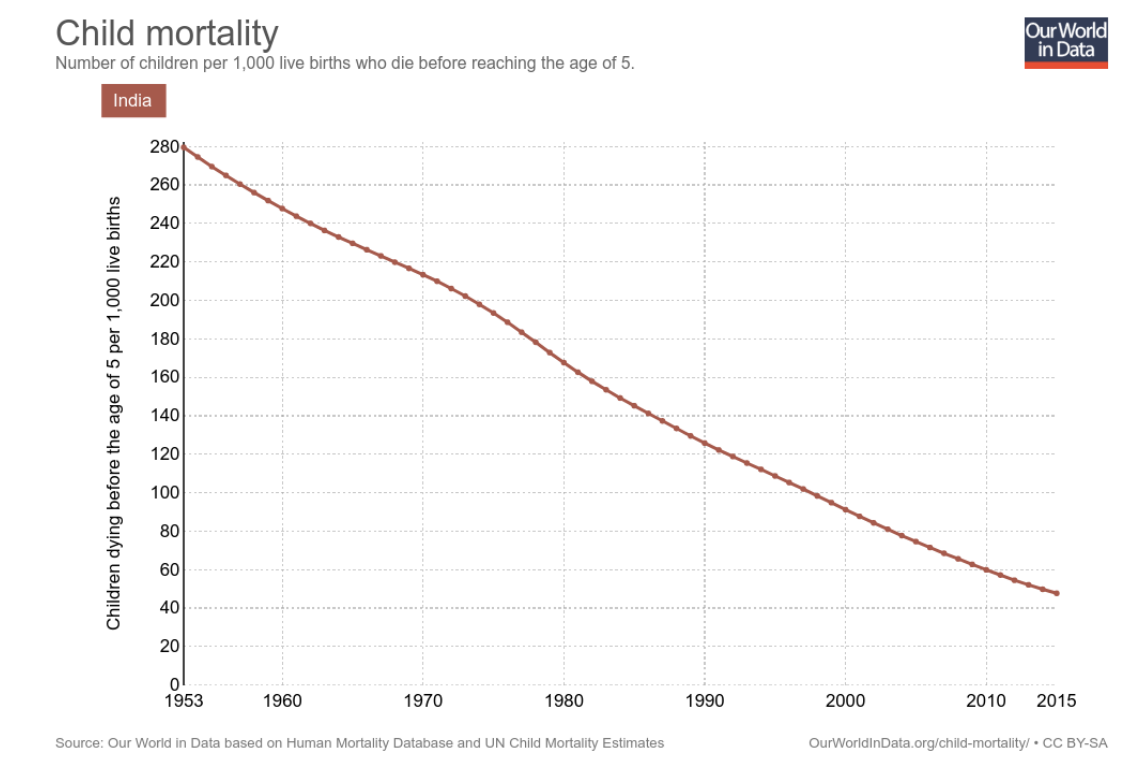
\includegraphics[scale=0.5]{InverseFunction}
%%	\end{center}
%\end{itemize}
%
%%%The amount of material that I have was not enough to fill 3 days. As a result I will add some here for the third day class.
%
%\newpage
%\subsection*{Problems to present at the board}
%The students will get into groups of 3. Each group will take a portion of the board or a white board from me. The students will then have approximately 5 minutes to complete their problem. When I call time, I will have the groups switch with a group near them. In a different color, the students will annotate and correct what they see on the board. They then will get together and discuss the corrections that they made to each others. Time permitting we will do this again with different problems. The following are the problems that the students will work with.
%
%\begin{itemize}
%	\item $f(x)=\frac{3x-2}{x+5}$
%	\item $g(x)=\frac{5x-10}{4x+7}$
%	\item $h(x)=\frac{2x-7}{10-5x}$
%	\item $k(x)=\frac{7x-11}{5-x}$
%	\item $f(x)=7x^3-4$
%	\item $g(x)=12x^5-13$
%	\item $h(x)=\frac{1}{2}x^7-11$
%	\item $k(x)=\frac{2}{3}x^3-8$
%	\item $f(x)=\frac{x-7}{7x-2}$
%	\item $g(x)=\frac{3x+4}{2x-12}$
%	\item $h(x)=\frac{7x+13}{12x+4}$
%	\item $k(x)=\frac{2x-1}{9x+11}$
%	\item $f(x)=9x^3+11$
%	\item $g(x)=7x^5-2$
%	\item $h(x)=\frac{3}{5}x^7+11$
%	\item $k(x)=\frac{2}{3}x^3+15$
%\end{itemize}
%
%\subsection*{Extra Practice Problems}
%Complete the following problems:\\
%\begin{enumerate}
%\item Find the inverse of $f(x)=\frac{6x+2}{4x-5}$
%\item Let $f(x)$ be a one-to-one function. What point must be on the graph if $f(9)=11$?
%\end{enumerate}

%%%%%%%%%%%%%%%%%%%%%%%% Quadratic Functions %%%%%%%%%%%%%%%%%%%%%%%%%%%

%\section*{Quadratic Functions}
%\subsection*{Introductory Example}
%A business has created a mathematical model based on market data for its profit, $P$ (in dollars), as function of the number of items sold, $x$. The model is given by the function \[ P(x)=-0.1x^2+150x-1400.\] How many units must be sold to maximize profit? What is the maximum profit?\\
%
%\noindent
%\textit{Students will work on this question with their partners. It is hoped that the students will graph it on their graphing calculator. To help them with the graphing calculator they should use the table feature to identify the zeros. Most students will probably use the maximize feature on their calculator. To hold them all accountable, I am going to ask each pair of students to write the window that they used on a whiteboard and hold it up for me to see the window. This way I know which students I should target to come to my office for extra help.} \\
%
%\noindent
%Some questions to ask students:
%\begin{enumerate}
%	\item What is the shape of this function? How would you describe it to someone?
%	\item Does the parabola have a maximum or minimum? What is it? 
%	\item What does the first coordinate of the vertex represent? The second coordinate?
%	\item How can we identify this point using just the equation, without the graph? \textit{This will be useful as some of the students are struggling with finding appropriate windows}
%	\item What is the relationship between the zeros and the vertex?
%	\item What is the formula for finding a vertex?
%\end{enumerate}
%
%\subsection*{Things you need to know about Quadratic Functions}
%\textit{In general quadratic functions are always parabolas and are symmetric about the vertex.}\\
%
%\noindent
%\textbf{General form: $f(x)=ax^2+bx+c$}\\
%\textit{$a$ is the leading coefficient, $a>0$ opens up, $a<0$ opens down, y-intercept $(0,c)$, vertex at $x=-\frac{b}{2a}$ to find $y$-coordinate plug in $x$ and solve.}\\
%
%\noindent
%\textbf{Vertex form: $f(x)=a(x-h)^2+k$}\\
%\textit{Think of this as a transformation of $y=x^2$, $a$ does the same thing as above, vertex $(h,k)$}\\
%
%\noindent
%\textbf{Factored form: $f(x)=a(x-r_1)(x-r_2)$}\\
%\textit{$a$ does the same thing as above, zeros: $r_1$, $r_2$,  $x$-coordinate of the vertex $\frac{r_1+r_2}{2}$}
%
%\subsection*{Practice Problems}
%$f(x)=2x^2+5x+3$\\
%
%\noindent
%Describe the following features of the quadratic function. 
%\begin{itemize}
%	\item The shape
%	\item $y$-intercept
%	\item Write it in vertex form
%	\item Write it in factored form
%\end{itemize}
%
%\noindent
%Find a formula for the parabola that goes through the points $(-5,0)$, $(3,0)$ and $(4,12)$\\
%\noindent
%\textit{If students are struggling, ask them to sketch a graph of it. Then ask them what form fits best based on what we were given. Have them find the vertex (x-coordinate).}
%
%\subsection*{Example 1}
%A concert venue holds a maximum of 1,000 people with ticket prices at \$30, the average attendance is 650 people. It is predicted that for every dollar the ticket price is lowered approximately 25 more people will attend. Create a function to represent the revenue generated from ticket sales and use this to find the maximum possible revenue.\\
%
%\noindent
%\textit{I want students to work and struggle with this problem on their own for a bit. This is similar to questions that they will be asked to do on the test so using their brains and thinking about it for a bit will be useful to them. I anticipate that the students will have a hard time with this problem, so some questions to have prepped to ask them follow here.}\\
%
%\noindent
%Some questions to ask stuck students:
%\begin{itemize}
%	\item How do you find revenue in this problem?
%	\item Make a table to find an equation for the price and average attendance. 
%	\item Can you find a function that represents attendance based on price?
%	\item Now use your equation for attendance and what you told me before to find your equation for Revenue.
%	\item How do you find the maximum revenue? What ticket price should be used to maximize revenue?
%\end{itemize}
%
%\subsection*{Example 2}
%Suppose a sunglass manufacturer determines the demand function for a certain line of sunglasses is given by $p=50-\frac{1}{4000}x$, where $p$ is the price per pair, and $x$ is the number of pairs sold. The fixed cost of producing this line of sunglasses is \$25,000 and each pair of sunglasses costs \$3 to produce. How many pairs of sunglasses should be produced and sold in order to maximize profits?\\
%
%\noindent
%\textit{Again I want students to work through this on their own, thinking about Revenue, Profit, Cost will be very helpful for the students during the exam. }\\
%
%\noindent
%A couple of questions to ask the students:
%\begin{itemize}
%	\item How do we find profit?
%	\item Can you write an equation for the cost?
%	\item Can you write an equation for the revenue?
%\end{itemize}
 
%%%%%%%%%%%%%%%%%%%%%%%% Polynomial Functions %%%%%%%%%%%%%%%%%%%%%%%%%%%

%\section*{Polynomial Functions}
%\subsection*{Opening Activity}
%We begin with an activity geared towards students discovering different aspects of the polynomial functions some basic graphs i.e. $x$, $x^2$, $x^3$, $x^4$, and $x^5$, and then more advanced graphs to help the students understand what multiplicity gives us in the graphs, as well as how different multiplicities affect zeros. \textit{The worksheet can be found in the concept check print-offs} \\
%
%\subsection*{Things to know about Polynomial Functions}
%At this point in time the students have filled out the worksheet and I will give them time to think about the following questions:
%\begin{itemize}
%	\item How does the degree of a polynomial function affect the ends of the graph?
%	\item How does the leading coefficient affect the ends of the graph?
%	\item What generalization can you make about the ends of the graph based on the degree of the polynomial and the leading coefficient?
%	\item How does the degree of the polynomial relate to the number of zeros it has?
%	\item How does the degree of the polynomial relate to the number of turns a graph has?
%\end{itemize}
%
%\noindent
%Things to know about Polynomial Functions:
%\begin{itemize}
%	\item General Form of a polynomial function \textit{make sure to talk about the degree, coefficients, and leading coefficients}
%	\item The leading term (degree and coefficient) tells us about the end behavior (long term behavior): \textit{Even/Odd and Positive/Negative, draw and dance}
%	\item The leading term tells us about the number of zeros and the number of turning points: \textit{number of zeros: $\leq$ degree, number of turns: $\leq$ degree minus one}
%	\item Finding zeros in factored form: \textit{if $(x-a)$ is a factor then $x=a$ is a zero}
%\end{itemize}
%
%\subsection*{Working time}
%At this point in time the students should have a good feel for polynomial functions. What they need to do at this point is to practice what they have learned. We will start with some basic examples (having students create equations from graphs and graph equations), we will then move into more complicated word problem examples.
%\begin{enumerate}
%	\item Determine the degree, leading coefficient, and zeros of the following polynomial equations. Sketch a rough graph by hand and check your answers on your graphing calculator. \begin{enumerate}
%	\item $y=x^3-x^2-6x$
%	\item $y=-\frac{1}{2}(x+3)(x-2)(x+1)(x-5)$
%	\item $y=-x^4+13x^2-36$
%	\end{enumerate}
%	\item Determine a possible equation for the following graphs. Verify your answers on your graphing calculator. \begin{enumerate}
%	\item 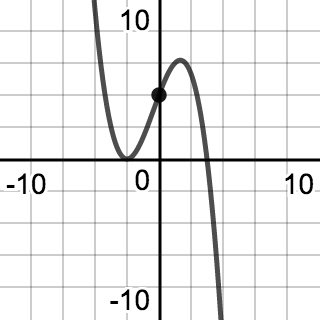
\includegraphics[scale=0.25]{cubicpractice.png}
%	\item 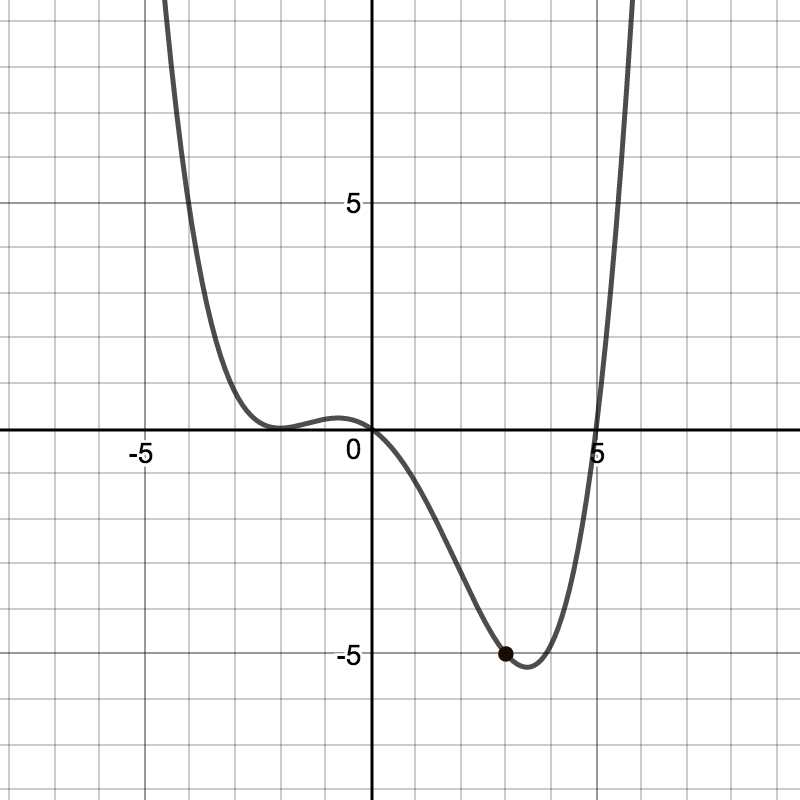
\includegraphics[scale=0.15]{quarticpractice.png}
%	\end{enumerate}
%	\item Based on actuarial life tables, the average number of years of life remaining for a female of age $x$ (up to 100) can be approximated by the function \[N(x)=0.0000004x^4-0.00004x^3+0.002x^2-1.0191x+81.955.\] Use this to answer the following questions: \begin{enumerate}
%	\item Graph this function in an appropriate window.
%	\item What does this graph tell us in practical terms?
%	\item What is the $y$-intercept? What does it mean in practical terms?
%	\item What is the degree of this function?
%	\item What is the leading coefficient of this function?
%	\item Is this function increasing or decreasing on the implied domain? What does this tell us in practical terms?
%	\item Why does it make sense that life expectancy increases as the age of the female increases?
%	\end{enumerate}	
%	\item A $12 \times 8$ rectangular piece of cardboard is folded into an open top box. This is possible by cutting squares from each of the corners. \begin{enumerate}
%	\item Determine a formula for the volume of the box.
%	\item Find the maximum possible volume.
%	\end{enumerate}	
%	\item For a particular pair of sunglasses, it is determined that the cost function is given by \[C(x)=0.00003x^3+7x+1,500\] and the revenue function is given by \[R(x)=-0.01x^2+40x\] where $x$ is the number of sunglasses produced and sold. Find a function to represent the profit as a function of $x$. Determine the number of units that should be sold in order to maximize profit. What is the maximum profit? 
%\end{enumerate}
%
%\noindent
%This should be enough material for at least two days. These last examples I am going to try to have the students work on them in their groups of three and will have them present as we go along. It should be a good productive struggle as they work through these problems with prompting from me.

%%%%%%%%%%%%%%%%%%%%%%%% Rational Functions %%%%%%%%%%%%%%%%%%%%%%%%%%%
%\section*{Rational Functions}
%\subsection*{Introductory Example}
%A clothes dryer is purchased for \$750, and electricity to run it costs approximately \$95 per year. Write a function that represents the average cost per year of operating the dryer. Graph this function in an appropriate window.\\[2mm]
%\textit{The students will definitely be able to write this function as a total cost function. It will probably take some prodding to get the students to think about average cost. (Have some questions in your back pocket about this). Creating the function is where I will have the students stop to verify they all have the appropriate equation. After they all have the appropriate equation we will discuss how to graph it in an appropriate window through filling in a table with $x$-values: $5, 10, 25, 40$. As we sketch the graph we will make sure to discuss the domain $(0,\infty)$ and the horizontal asymptote $y=95$}
%
%\subsection*{Things to know about Rational Functions}
%General form: \textit{A rational function has the form $f(x)=\frac{p(x)}{q(x)}$ where $p(x)$ and $q(x)$ are polynomial functions}\\[2mm]
%Domain of a rational function: \textit{Remove all the $x$-values which make the denominator zero}\\[2mm]
%Zeros of a rational function: \textit{The $x$-values for which the numerator is zero.}\\[2mm]
%Vertical Asymptotes: \textit{When the denominator is 0, we write $x=\underline{\hspace{1cm}}$. There is not always a vertical asymptote.}\\[2mm]
%Horizontal Asymptotes: \textit{Has a horizontal asymptote whenever the degree of the numerator is less than or equal to the degree of the numerator. It tells us the end behavior of the graph}
%
%\subsection*{Example to Practice with}
%\[f(x)=\frac{3x-2}{x-1}\]
%\textit{Students will identify: Domain, Zeros, Vertical Asymptote, Horizontal Asymptote}
%
%\textit{The next sections of things are warm-up and the remainder of the lecture material.}
%For the following function identify the domain and write equations for all the asymptotes. Verify your answer by graphing.
%\[f(x)=\frac{2x+1}{x^2-16}\]
%
%Find an equation for the following rational equations.\\
%\begin{center}
%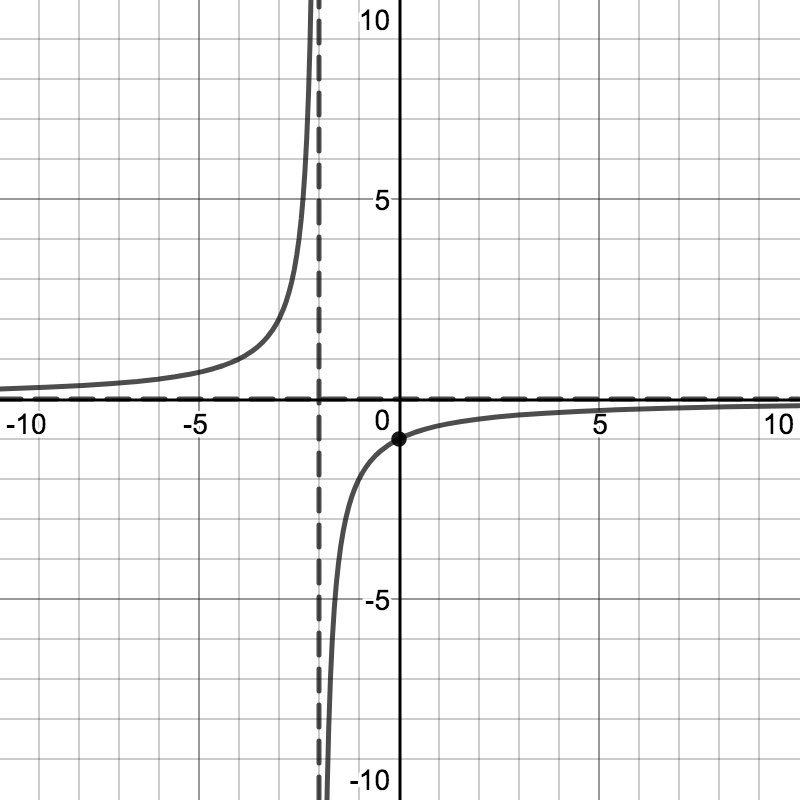
\includegraphics[scale=0.15]{graph2.png}\\[10mm]
%\end{center}
%
%\begin{center}
%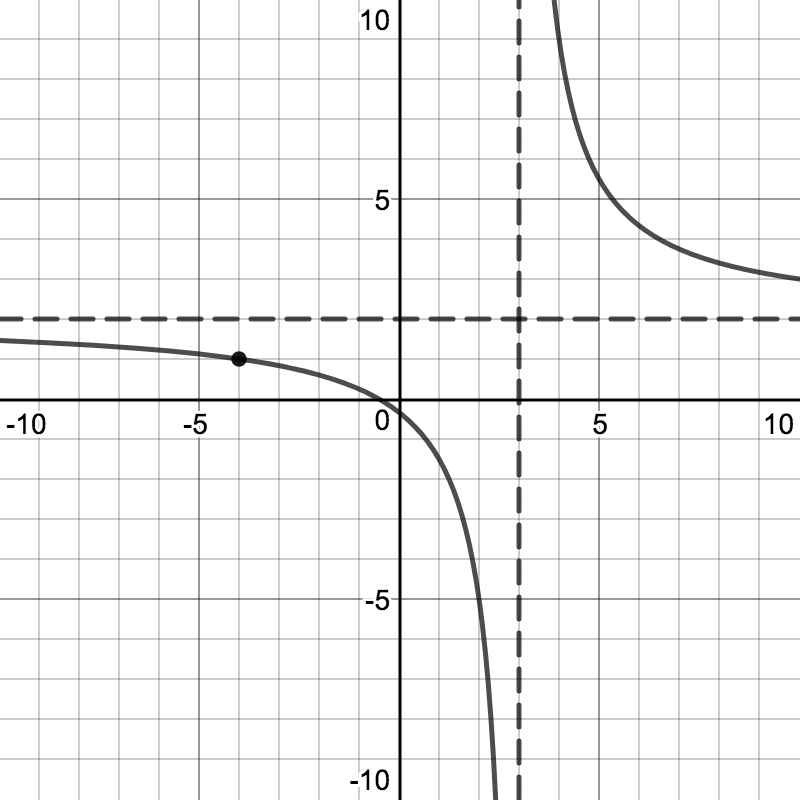
\includegraphics[scale=0.15]{graph1.png}
%\end{center}
%
%\noindent
%A company that assembles bicycles has determined that a new employee can assemble $M(d)$ bicycles per day after $d$ days of on-the-job training, where $M(d)=\frac{100d^2}{3d^2+10}$. After how many days of training would an employee be able to assemble 25 bicycles per day?\\[4mm]
%
%\noindent
%\textit{On day 3 students will work on problems. There will be 10 problems (equating to two rounds) for the students to work on. For the first ~10-15 minutes of class the students will work on one of the problems for the first set with a group of 5 students. At the end of the allotted working time the students will reorganize according to cards that I give them as they are working. In their groups they will take time to explain to each other how to solve the problem that they were giving. This should take about 10-15 minutes. We then will repeat the process. Potentially with the second round I will project the solutions to the problems.}
%\subsection*{Problem Set 1}
%\begin{enumerate}
%	\item Determine an equation for the rational function that has:
%		\begin{itemize}
%			\item $f(x)$ has a zero at $x=2$
%			\item $f(x)$ has a vertical asymptote at $x=-1$
%			\item $f(x)$ has a horizontal asymptote at $y=3$
%		\end{itemize}
%	\item A patient is being treated for a chronic illness. The concentration $C(x)$ in $g$ per $mL$ of a certain medication in the patient's bloodstream $x$ weeks after taking the medication is approximated by $C(x)=\frac{8x^2-31x+35}{4x^2-16x+17}$. During what week is the largest concentration in the patient's bloodstream? How much is in their bloodstream during that week? As time passes how much medication will be in the patient's bloodstream?
%	\item Answer the following questions about the rational function $f(x)=\frac{x^2+3x-18}{x^2-4}$. Identify the: 
%		\begin{itemize}
%			\item Domain
%			\item Vertical Asymptote
%			\item Horizontal Asymptote
%			\item Zeros
%			\item $y-$intercept
%		\end{itemize}
%	\item The cost $C$ in millions of dollars of removing $x\%$ of pollutant from a lake is given by $f(x)=\frac{50x}{100-x}$, where $0 \leq x \leq 100$. Use this information to answer these questions:
%		\begin{itemize}
%			\item Evaluate $f(60)$ and interpret what it means in context of the problem
%			\item If a company has 25 million dollars to spend how much pollutant can they remove?
%			\item What amount of money does a company need to have in order to remove 95\% of the pollution?
%			\item A current law states that in order for a state to receive federal funding at least 10\% of the funding must be utilized clean water ways. If the government is funding 900 million to a certain state how much pollutant can they remove from the lake?
%		\end{itemize}
%	\item The number of random facts a person can learn depends on the number of minutes, $m$, they spend studying. This is represented by the following graph. Use the graph to find an equation that represents the number of facts a person can learn. 
%		\begin{center}
%			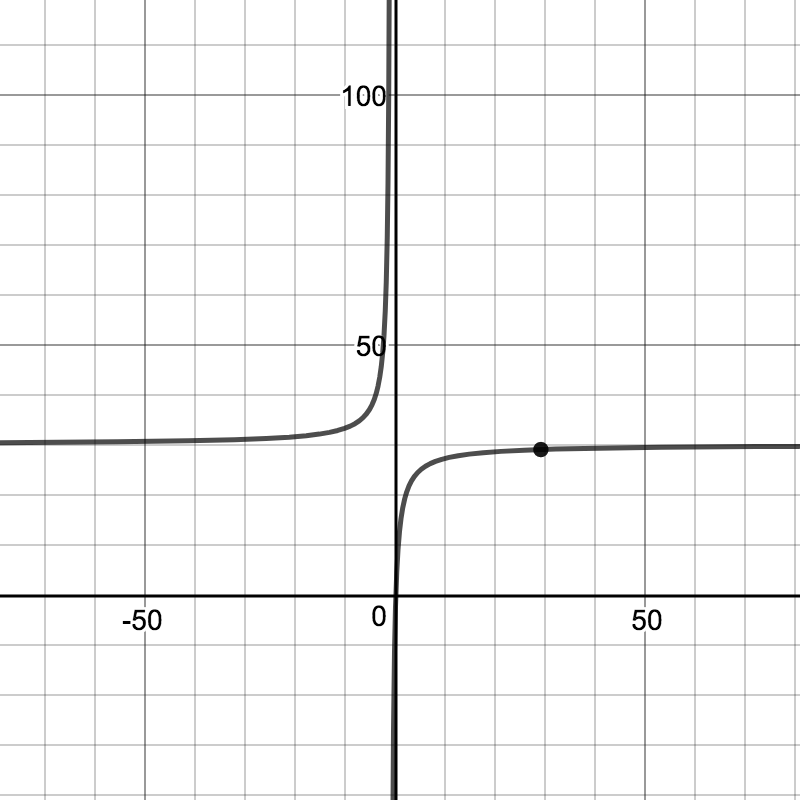
\includegraphics[scale=0.25]{rationalfunction3}
%		\end{center}
%\end{enumerate}
%
%
%\subsection*{Problem Set 2}
%\begin{enumerate}
%\item A company that produces telephones has determined that the monthly fixed cost is \$12,000 and it costs \$30 to manufacture each telephone. Use this information to answer the following questions.
%	\begin{itemize}
%		\item Write a function that represents the average cost per telephone.
%		\item Determine an appropriate domain for the function.
%		\item As the number of telephones the company produces increases, what does the average cost become?\\[4mm]
%	\end{itemize}
%	
%\item A scientist is studying the temperature in a certain region of a remote planet. She approximates the temperature, $T$ in degrees Celsius in that region $x$ years after the planet's origin to be the following $T=\frac{3x^2-13x+8}{x^2-4x+8}$. In what year was the temperature the coolest? What was the coolest temperature? Does the temperature of the planet ever level off? If so, what does the temperature tend to?
%
%\end{enumerate}

%%%%%%%%%%%%%%%%%%%%%%%% Exponential Functions %%%%%%%%%%%%%%%%%%%%%%%%%%%

%\section*{Exponential Functions}
%\subsection*{Warm-Up}
%Let's talk about rabbits $\cdots$\\[4mm]
%\begin{tabular}{c|c}
%Time & Number of Rabbits \\ \hline
%0    & 2                 \\
%1    & 6                 \\
%2    & 18                \\
%3    & 54                \\
%4    & 162               \\
%5    & 486              
%\end{tabular}\\[4mm]
%
%\noindent
%\textit{The students will work on this as a warm-up problem. My directions to them will be to first find the pattern. After they have found the pattern I will have them come up with an equation to represent the situation after	 time $t$.}\\
%
%\subsection*{Introductory Example}
%Nathan has \$100 to open a savings account. He found an account that offers 2.5\% interest compounded annually. Write a function to represent the balance in the account as a function of time in years, assuming the initial deposit and all subsequent interest is kept in the account. Graph this function in an appropriate window.\\
%\textit{This is an example we will work on as a class to accomplish. We will do so by creating a table with one column that represents the years and the other column that represents the amount of money in the account and work from there}
%
%\subsection*{Things to know about Exponential Functions}
%What is the general form of on exponential function? \textit{$f(x)=C \cdot b^x$ where $C$ is the $y$-intercept (any real number) $b>0$, $b \neq 1$}\\
%What differentiates an exponential function from the other types of functions we have studied? \textit{variable is in the exponent}\\
%What is the domain of an exponential function? The range? The intercept(s)? The asymptote(s)? \textit{Pictures if $b>1$, $0<b<1$ Domain: $(-\infty, \infty)$, Range: $(0,\infty)$ if $C>0$, $(-\infty, 0)$ if $C<0$. }\\
%What determines whether an exponential function is increasing or decreasing? \textit{Increasing if $b>1$, decreasing if $0<b<1$}\\
%What is the formula for compound interest if it is compounded annually? $n$ times per year? continuously? \textit{$A=P(1+r)^t$, $A$ is the final amount, $P$ is the Principle (initial) amount $A=P\left(1+\frac{r}{n}\right)^{nt}$, $n$ is the number of times per year.}\\
%
%\subsection*{A warm-up for day 2}
%Determine the for $y=C \cdot b^x$ that passes through the points $(1,12)$ and $(3,192)$.
%
%\subsection*{Example 1}
%A person plans to invest \$5,000 into a money market account. Find the interest rate required for the money to grow to \$45,000 in 30 years if the interest is compounded quarterly.
%
%\subsection*{Example 2}
%Bacteria from raw eggs has come into contact with the onions and celery you are going to put into your potato salad. Initially there were 500 bacteria present; one hour later there were 4,000 bacteria present in the salad. The population of the bacteria in the salad can be modeled by a exponential function $y=C \cdot b^t$, where $t$ is measured in hours. Create a function that represents this situation, and use the graph to determine the number of hours it takes for the bacteria's population to double in size.
%
%\subsection*{Example 3}
%\$100 is invested into an account bearing 12\% interest. What will the balance in the account be in 10 years if $\ldots$\\
%interest is compounded annually?\\
%interest is compounded quarterly?\\
%interest is compounded monthly?\\
%interest is compounded daily?\\
%
%\noindent
%\textit{This example leads to continuously compounding $A=Pe^{rt}$, where $e=2.718281828459045\ldots$.}
%
%\subsection*{Example 4}
%A radioactive substance has a half-life of 20 days. If the initial amount is 25 grams, write a function to represent the amount of substance remaining after $t$ days.\\
%
%\noindent
%\textit{This example can be done either using $A=Pe^{rt}$ or $y=C\cdot b^t$. The best way to approach this problem is to have students do it both ways. Split the room down the middle and have the students on the left hand side use $A=Pe^{rt}$ and the other students use $y=C\cdot b^t$ and come back and share to see that we get the same output regardless of which we use.}

%%%%%%%%%%%%%%%%%%%%%%%% Logarithms %%%%%%%%%%%%%%%%%%%%%%%%%%%

%\section*{Logarithms}
%\subsection*{Introductory Example}
%\$1 is invested in an account earning 5\% interest compounded annually. How long will it take the amount in the account to grow to \$2.
%
%\noindent
%\textit{The students will work on this problem on their own. By this point in time I anticipate that they will have worked on these ideas on their own through a couple of exponential problems that they can use their calculators to estimate. I hope that one of them will come up with the same idea here.}
% 
%\subsection*{Introductory Example 2}
% Once the students have worked on this I will ask them the following questions as a class about the example $y=2^x$: 
% 
% \begin{itemize}
% 	\item If I gave you a $y$ value, could you solve the question algebraically?
% 	\item Does the function have an inverse?
% 	\item How do you know?
% 	\item Create a table of values for the inverse function.
% 	\item Sketch a graph of the inverse.
% 	\item What is the domain, range, intercept(s) and asymptote(s) for the inverse function?
% \end{itemize}
% 
% \noindent
% \textit{Once we have gone through the example together, we will show the equivalence between $y=2^x$ and $x=\log_2(y)$. They are inverses! We shouldn't be scared because we know how to handle them}
% 
% \subsection*{Things to know about logarithmic functions}
% 
% \begin{enumerate}
% 	\item What is a logarithm? \textit{The inverse of an exponential equation}
% 	\item What is the notation for logarithm? What is the exponential equivalent of a logarithm? \textit{$\log_b(y)=x$ means $b^x=y$}
% 	\item How do you evaluate simple logarithmic expressions? \textit{solve $\log_2(8)=x$}
% 	\item What is the common logarithmic function? The natural logarithmic function? \textit{$\log(x)=\log_{10}(x)$ common log, $\ln(x)=\log_e(x)$ natural log}
% 	\item What is the domain/range/intercept/asymptote of a logarithmic function? \textit{$f(x)=\log_b(x)$ Domain: $(0,\infty)$, Range: $(-\infty,\infty)$, $x$-intercept: $(1,0)$, V.A. at $x=0$ }
% \end{enumerate}
%
%\subsection*{A good computational example}
%Find the domain and intercepts of the logarithmic function, and sketch the graph $f(x)=\log(3x-2)$.\\
% 
%\noindent
%\textit{This is a good example for the students to do to see that the domain of a logarithm is defined by what is in the parentheses. Namely, the input must not be negative. It is also good practice to get some computation down before jumping back into word problems. Make sure to emphasize that the domain is dependent on the input to the logarithm being non-negative.}
%
%\subsection*{Example 1}
%The amount of radioactive material in a 200-gram sample of bismuth can be modeled by the function $A(t)=200e^{-0.1386t}$, where $t$ is time in days. What is the half-life of this radioactive material?\\
%
%\noindent
%\textit{This example is one to go through with the students most likely. I will try to have them do it on their own but it will probably be challenging. When you do go through it make sure to do it in the following way.}
%
%\begin{align*}
%	200e^{-0.1386t} &= 100\\
%	e^{-0.1386t} &= \frac{1}{2}\\
%	\log_{e}(0.5) &= -0.1386t\\
%	\frac{\ln(0.5)}{-0.1386} &= t
%\end{align*}
%
%\subsection*{Example 2}
%A population of 1000 bacteria is on the kitchen counter. The amount of time, in hours, that it takes the population to reach $x$ bacteria is given by $f(x)=16 \cdot \ln\left( \frac{x}{1000}\right)$. How many bacteria will their be in 3 hours. \\
%
%\noindent
%\textit{For this problem students will need to rewrite the problem in exponential form and solve for $x$ in that way. If we run out of material we can go back to the first problem and try to solve that one algebraically now that we know how to do so.}

%%%%%%%%%%%%%%%%%%%%%%%% Properties of Logarithms %%%%%%%%%%%%%%%%%%%%%%%%%%%

\section*{Properties of Logarithms}
\subsection*{Introductory Example}
\textit{For the introduction to this section the students will work on a worksheet to come up with the common rules for logs ``multiplication turns into addition" etc. The students will compute this without using their calculators as it will be good practice for them to turn the logs into exponentials and reason their way through the problems since we technically don't know change of base.}

\subsection*{Things to know about the Properties of Logarithms}
What is the property for a logarithm of an input that is multiplied? \textcolor{blue}{$\log_b(x \cdot y)=\log_b(x)+\log_b(y)$}  \\
What is the property for a logarithm of an input that is divided? \textcolor{blue}{$\log_b \left(\frac{x}{y}\right) = \log_b(x)-\log_b(y)$} \\
What is the property for a logarithm of a power? \textcolor{blue}{$\log_b(x^p)=p \cdot \log_b(x)$ } \\
What is the inverse property of logs/exponential functions?\textcolor{blue}{$f(x)=b^x$ and $g(x)= \log_b(x)$ are inverses of each other so \ldots $(f \circ g)(x)=x$ and $(g \circ f)(x)=x$ go through the steps to get these results}\\

\subsection*{Practice Practice Practice}
\textit{The remainder of the class will be spent workin on using these properties productively and correctly. I most likely will have the students work in small groups on these problems and will have the students present their solutions to each other and have them tell me what to do next as we go through them}\\

\noindent
Use the properties of logs to rewrite the following as a single logarithmic expression:\\

\noindent
$\ln(6x)+\frac{1}{2}\ln(x)-\ln(2x)$\\

\noindent
$\log(5z)-\log(x)-3\log(3y)+\log(t)$\\

\noindent
$2log_2(x^2)+\log_2(y)-4\log_2(P)-\frac{1}{3}\log_2(Q)+\log_2(z)$\\

\noindent
Use the properties of logarithms to expand each expression as much as possible:\\

\noindent
$\ln(10xe^3x)$\\

\noindent
$\log\left(\frac{2x^4}{y\sqrt{z}} \right)$\\

\noindent
$\log_5(\sqrt{5z})$\\

\noindent
A couple more problems to try:\\

\noindent
Use the natural logarithm and a property of logarithms to solve: $4(3)^x=20$.\\

\noindent
Use property of logarithms to solve:\\

\noindent
$\log(-x-2)+\log(1-x)=1$\\

\noindent
$\log_3(3x+17)-\log_3(x+1)=2$





\end{document}






































